\documentclass[a4paper,fontset = windows]{ctexbook}
\usepackage{xifthen}
\usepackage{calc}
\usepackage{graphicx}
\usepackage{tikz}
\usepackage[user=student,option=random]{cexam}
\usepackage[fontwarning=on]{ctrlwarning}

\begin{document}
\chapter{选择题选项排版测试}

 \begin{choices}
   2.选择题题干,如果插入图片,则图片应当如所示.
    从下面四个选项中选出正确的选项
    \choice[A]{错误选项}
    \choice[B]{错误选项}
    \choice*[C]{正确选项原因未知}
    \choice*[D]{正确选项都是老师}

    a.*

    e.答案是\refc{}未知,\refd{}是老师。

   2.选择题题干,如果插入图片,则图片应当如所示.
    从下面四个选项中选出正确的选项
    \choice[A]{错误选项}
    \choice[B]{错误选项}
    \choice*[C]{正确选项原因未知}
    \choice*[D]{正确选项都是老师}

    a.*

    e.答案是\refc{}未知,\refd{}是老师。

   2.选择题题干,如果插入图片,则图片应当如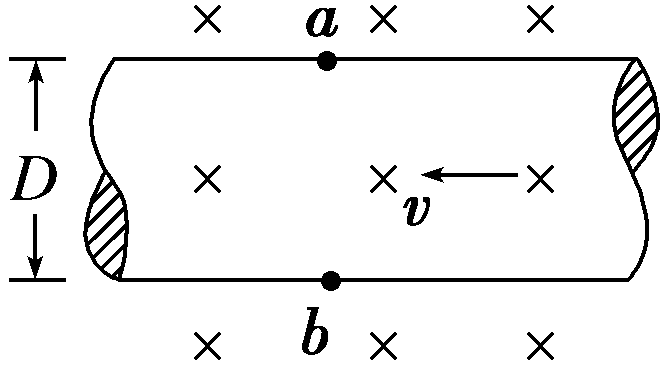
\includegraphics{1.png}所示.
    从下面四个选项中选出正确的选项
    \choice[A]{错误选项}
    \choice[B]{错误选项}
    \choice*[C]{正确选项原因未知}
    \choice*[D]{正确选项都是老师}

    a.*

    e.答案是\refc{}未知,\refd{}是老师。

 \end{choices}


\ExplSyntaxOn
\bool_case_true:n
{
   {
      \dim_compare_p:n 
      {1pt=1pt<3pt}
   }
   {Hello}
   {\dim_compare_p:n {1pt=2pt}}{Good}
}
\ExplSyntaxOff


\makeanswer

\end{document}
